\subsection{Pharmacokinetics \& Pharmacodynamics}

In this section, I describe pharmacokinetic and pharmacodynamic theory as it will be used in the proposed research.  I will explain aspects of both pharmacokinetic and pharmacodynamic models, and how the two are related.  One and two compartment model(s) for pharmacokinetics will be constructed and interpreted.


\subsubsection{Pharmacokinetics v. Pharmacodynamics}

The phases between drug administration and emergence of the desired effect can be broadly placed into one of two areas of study.  The area of study which is concerned with relationship between dose administration and achievement of particular concentrations in the body is known as \textit{pharmacokinetics}, while the area of study concenred with the arrival of the drug at it's site of action, the onset of the desired effect, as well as the magnitude and duration of that effect is known as  \textit{pharmacodynamics} \cite{rosenbaum2016basic}.  

\subsubsection{A One Compartment Pharmacokinetic Model}

To analyze the time course of drug concentrations in various parts of the body, compartmental models are often used.  These models posit that the body (or relevant organs/systems of the body) is comprised of compartments from which drug can flow in and out. The rates at which the drug can enter and exit each compartment are specified, and a differential equation for each compartment can be created and solved.

The simplest example of these models is the one compartment pharmacokinetic model.  A bolus dose of a drug is administered to the patient and the drug is absorbed from the gut into the blood.  Here, the gut and the blood form two compartments, but we are not usually interested in concentrations of drug in the gut, and so we usually focus only on the concentration of drug in the blood (hence, one compartmental model).  A visual representation of this model is shown in \cref{compartmental_model}.

\begin{figure}[h!]
	\centering
	
	\tikzstyle{int}=[draw, fill=white, minimum size=2em]
	\tikzstyle{init} = [pin edge={to-,thin,black}]
	
	
	\begin{tikzpicture}[node distance=2.5cm,auto,>=latex']
	
	
	\node [int] (a) {$G$};
	\node (b) [left of=a,node distance=2cm, coordinate] {a};
	\node [int] (c) [right of=a] {$C$};
	\node [coordinate] (end) [right of=c, node distance=2cm]{};
	\path[->] (a) edge node {$k_a$} (c);
	\draw[->] (c) edge node {$k$} (end) ;
	\end{tikzpicture}
	\caption{A compartmental diagram for a one compartment pharmacokinetic model.}
	\label{compartmental_model}
\end{figure}

In this diagram, $ G $ is the compartment for the gut, and $ C $ is the compartment for the blood.  Both $ G $ and $ C $ represent the concentrations of drug in gut and blood respectively.  The drug leaves the gut ($ G $) and enters the blood ($ C $) at rate $ k_aG $.  The drug is then excreted from the body at rate $ kC $.  The system can be written as a differential equation, namely,
%
\begin{alignat*}{3}
	\dfrac{dG}{dt} &= -k_aG \>, \quad  &&G(0) = \dfrac{D}{V} \\
	\dfrac{dC}{dt} &= k_aG - kC \>,   \quad  &&C(0) = 0
\end{alignat*}
%
Here, $D>0$ is the dose size and $V>0$ is the volume of the gut.  It can be shown that the solution for the concentration of drug in the blood at a given time is 

\begin{equation}\label{onecompartment_PKPD}
	C(t) = \dfrac{D}{V}\dfrac{k_a}{k_a - k}\Big(e^{-k_at} - e^{-kt}\Big) \>.
\end{equation}

\begin{figure}[h!]
	\centering
	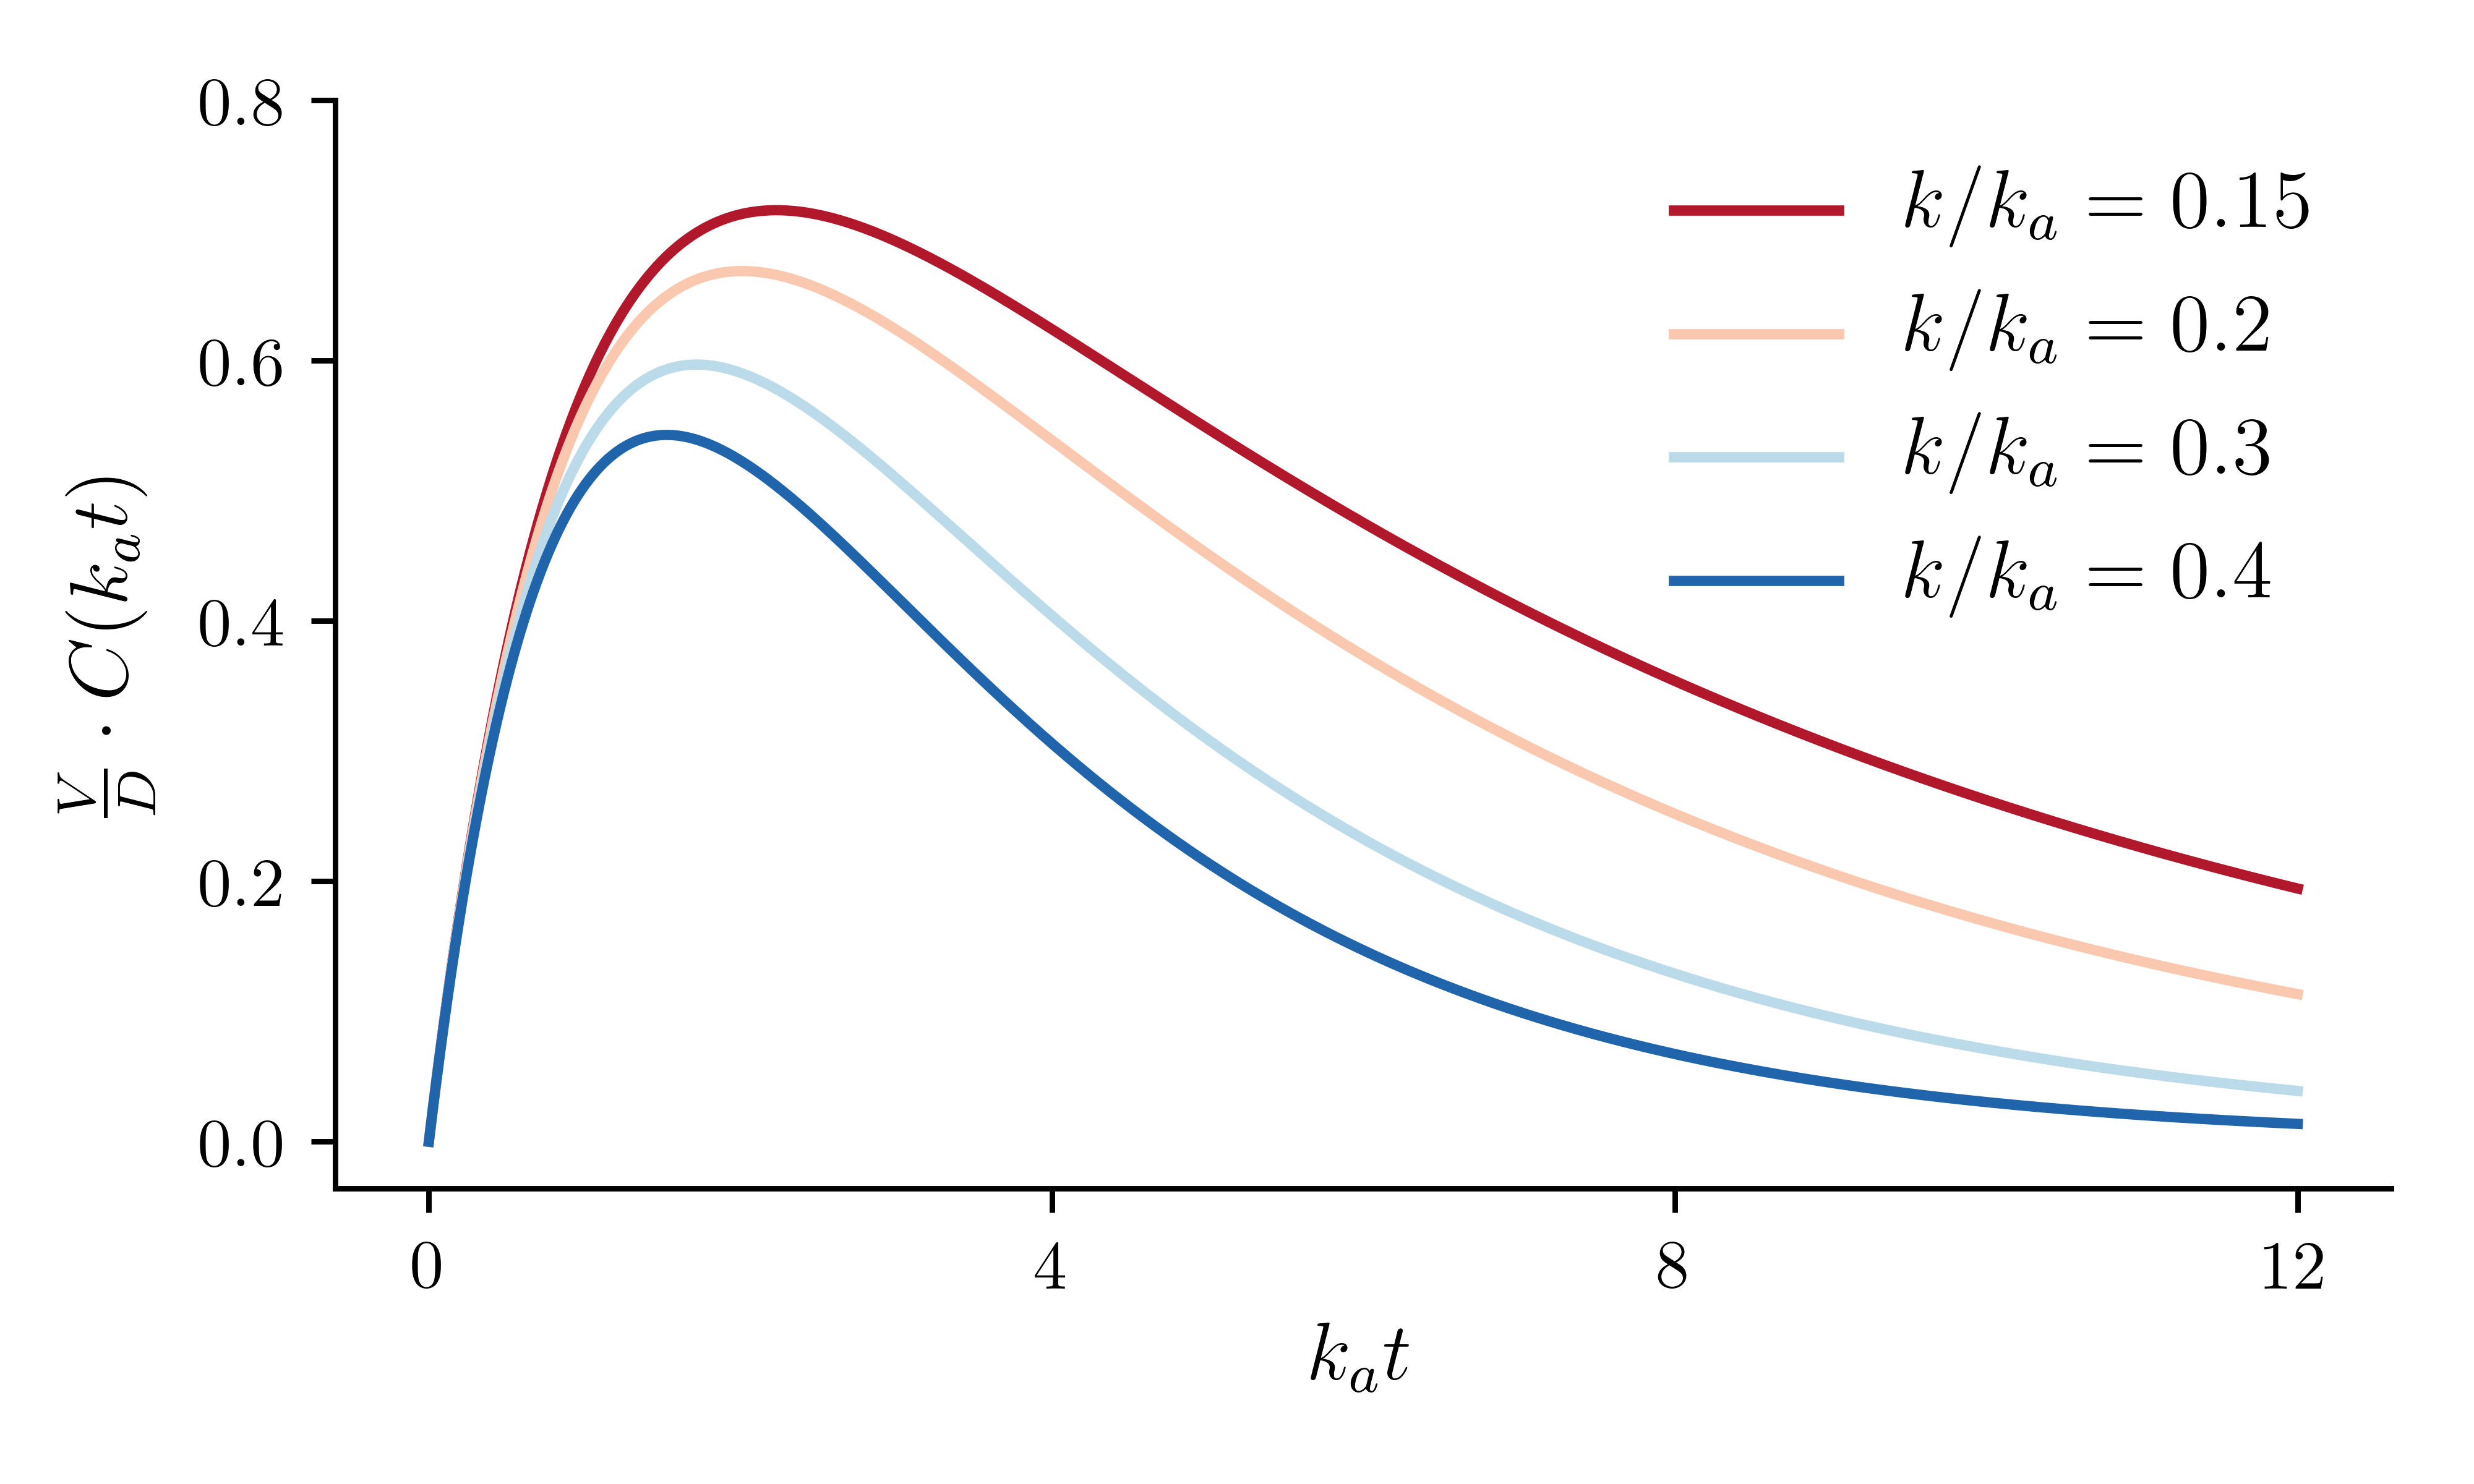
\includegraphics{Figures/pkcureves.png}
	\caption{Plots of \cref{onecompartment_PKPD} under various parameterizations.  Holding $D/V$ constant and examining various values of $k/k_a$ leads to curves shown.  The time scale has also been altered so as to account for varying rates of drug influx/outflux.  This process is called \textit{non-dimensionalization}, and is often used in the analysis of dynamical systems.  We see that as $\frac{k}{k_a} \rightarrow 1^-$, the maximum concentration of drug in the blood shrinks, and the drug exists the body much faster.}
	\label{fig:pkcureves}
\end{figure}


\subsection{A Two Compartment Pharmacokinetic Model}